\section{Localizing nomination uncertainty and separating arithmetic}
\label{sec:main-localization}

\begin{theorem}[Block-rank pressure and arc algorithms]
\label{thm:main-block}
Fix $r_0$. Let $G$ be connected with $r_{\max}\le r_0$, and let
nominations range over a nonempty balanced rational box.
For symmetric quadratic laws with independent positive rational
resistance intervals, every prescribed terminal-drop maximum satisfies
\eqref{eq:main-contract} in time polynomial in $N_\eps$ for fixed $r_0$.
Every individual arc has exactly computable algebraic minimum and
maximum of polynomial encoding length, so unfiltered robust signed
capacity validation is polynomial-time, including equality.

The same conclusions hold for laws affine in arbitrarily many independent
rational interval parameters, with densely encoded rational continuous
piecewise-polynomial basis functions vanishing at zero and fixed rational
breakpoints, provided every allowed complete law is strictly increasing.
Degrees and piece counts may grow. The pressure scenario output is
rational; the exact arc conclusion asserts algebraic values, without a
general rational near-extremal arc-output guarantee for these laws.
No additional operating bounds filter the nomination or coefficient
scenario domain in either assertion.
\end{theorem}

This combines \cref{thm:a-blk-joint,thm:a-blk-arc,thm:a-law-polynomial}.
For the independent affine-box representation, the dense-law
admissibility conditions can themselves be checked in polynomial time
(\cref{prop:a-law-validation}). The exponent depends on $r_0$ (an XP
bound); implicit laws and sparse binary exponents are not covered. By
\cref{prop:a-blk-limits}, based on
\citet{thurauf2022-deciding-the-feasibility-of-a}, block rank cannot be
replaced by treewidth two, series-parallel structure, or feedback vertex
number one unless $\mathrm P=\NP$, even with fixed resistances.

\subsection{Proof mechanism: adjoint levels and small faces}

The first reduction removes components outside the terminal block path
and sums their nomination intervals at the attachment vertices. Every
feasible aggregate has a rational disaggregation, obtained by filling
the original intervals from their lower bounds. Since the domain is
unfiltered, no operating constraint is lost.

Temporarily smooth the edge laws so their derivatives are positive.
Differentiating \eqref{eq:main-state} and pairing with the terminal
objective gives
\begin{equation}
 dF_{s,t}=h^\top db,\qquad
 A\operatorname{diag}(1/g'_e(x_e))A^\top h=e_s-e_t.
 \label{eq:main-adjoint}
\end{equation}
The adjoint $h$ is the potential of a unit electrical network. At a
maximum over a balanced box, a multiplier $\mu$ for balance exists such
that $h_v>\mu$ forces $b_v=u_v$ and $h_v<\mu$ forces $b_v=\ell_v$, so
only nominations at the level $h_v=\mu$ remain free. The maximum
principle strictly orders the adjoint ranges of consecutive blocks, so
one threshold meets internal vertices of at most one block.

On a cactus, the adjoint is strictly monotone down each of the two
branches of that block. At most two nominations remain free, one on
each branch, and balance leaves one parameter; there are $O(n^2)$
candidate faces. On a higher-rank block, mark the terminals and the
vertices of degree at least three, and suppress the degree-two paths
between them; there are at most $2r_B$ marks and $3r_B-1$ paths. A small
positive objective source at every unmarked vertex makes the electrical
current strictly increase along each path, so its potential is unimodal
and every threshold occurs at most twice. Enumerating the resulting
lower/free/upper/free/lower patterns leaves at most $8r_B-2$ free
nominations. Compactness and uniform convergence remove the smoothing
and perturbation; the algorithm enumerates closed faces and never
computes a perturbation size.

\begin{figure}[tb]
\centering
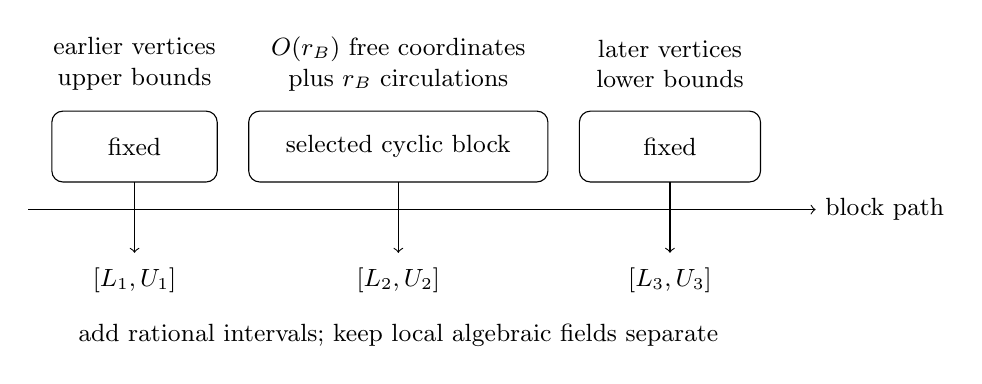
\begin{tikzpicture}[x=1cm,y=1cm,every node/.style={font=\small}]
\draw[->] (0,0)--(10,0) node[right] {block path};
\foreach \a/\b/\txt in {0.3/2.4/fixed,2.8/6.6/selected cyclic block,7/9.3/fixed}{
 \draw[rounded corners] (\a,.35) rectangle (\b,1.25);
 \node at ({(\a+\b)/2},.8) {\txt};}
\node[align=center] at (1.35,1.85) {earlier vertices\\upper bounds};
\node[align=center] at (4.7,1.85) {$O(r_B)$ free coordinates\\plus $r_B$ circulations};
\node[align=center] at (8.15,1.85) {later vertices\\lower bounds};
\draw[->] (1.35,.35)--(1.35,-.55);
\draw[->] (4.7,.35)--(4.7,-.55);
\draw[->] (8.15,.35)--(8.15,-.55);
\node at (1.35,-.9) {$[L_1,U_1]$};
\node at (4.7,-.9) {$[L_2,U_2]$};
\node at (8.15,-.9) {$[L_3,U_3]$};
\node at (4.7,-1.6) {add rational intervals; keep local algebraic fields separate};
\end{tikzpicture}
\caption{Nomination localization for a terminal difference. Independent
coefficients may still be optimized in every block; ``fixed'' refers to
aggregated nominations. The selected block is cyclic; bridge cases
are handled directly. The number of blocks is unrestricted.}
\label{fig:main-localization}
\end{figure}

The second reduction handles the many coefficient variables. Inside
a selected face, flow is affine in the free nominations and the
$r_B$ cycle circulations. On each flow-sign or law-piece cell, the
cycle equations are polynomial in this small core and affine in the
coefficient parameters, so the image of a coefficient box in the cycle
and objective coordinates is a zonotope of fixed dimension. Its support
inequalities can be expanded over the realizable sign patterns, which
are polynomially many at fixed dimension, and quantifier elimination
removes the remaining fixed-dimensional support variables. The leaf
coordinates are recovered from exposed zonotope vertices and a
fixed-size convex combination. This avoids enumerating all box corners;
the fact that an LP vertex has few non-bound coordinates would not by
itself give an efficient algorithm.

The fixed-dimension bounds are classical
\citep{renegar1992-on-the-computational-complexity-and,basu2006-algorithms-in-real-algebraic-geometry};
we keep the number of real variables bounded \emph{per block}, even
when law degrees and numbers of uncertain coefficients grow. Independent
block optima are enclosed separately and their rational intervals added.
A pressure sensitivity estimate then permits rational rounding inside
the original nomination and coefficient constraints. The proofs in
\cref{sec:a-block-rank,sec:a-laws} handle ties, zero flows, singleton
faces, degenerate polytopes, and output bit length.

\subsection{An exact arithmetic boundary on a chain of triangles}

\begin{theorem}[Cactus arithmetic and fixed fractional powers]
\label{thm:main-arithmetic}
For symmetric quadratic laws with fixed positive rational resistances,
MPD over a balanced rational nomination box on a cactus satisfies
\eqref{eq:main-contract} in polynomial time. On the restricted box
$b=\zeta(e_s-e_t)$, $0\le\zeta\le1$, exact weak threshold comparison
is polynomial-time many-one equivalent to Square-Root Sum. Hardness
holds on simple degree-three chains of triangles with positive integer
resistances.

For every fixed finite family $\mathcal Q\subset\Q\cap(1,\infty)$,
the laws $g_e(t)=\beta_e\sgn(t)|t|^{q_e}$, $q_e\in\mathcal Q$, admit
the additive value and rational-scenario contract for terminal drops
and individual arcs at fixed maximum block rank, over a balanced rational
nomination box and independent positive rational resistance intervals,
without operating filters. For any fixed reduced exponent greater than
one with even denominator, exact arc-capacity comparison is
Square-Root-Sum hard already on a single simple cycle with fixed integral
nominations and positive integral resistances.
\end{theorem}

The quadratic statements are \cref{thm:a-cac-additive,thm:a-cac-srs};
the power-law statements are \cref{thm:a-law-fractional,thm:a-law-srs}.
Square-Root Sum asks whether $\sum_i\sqrt{a_i}\le K$ for positive
binary integers $a_i,K$. Whether it is decidable in polynomial time, or
even lies in NP, is open (see also \citet[Section 5]{ajdarow2025-taming});
its known upper bounds are discussed in \cref{subsec:a-pre-computation}.

The arithmetic gadget uses a triangle whose two terminal branches have
total resistances $(a-1)^2$ and $(a-1)^2/a$ for $a\ge2$. Its unit-flow
drop is
\[
 R_a=a+1-2\sqrt a>0.
\]
Joining these triangles by unit bridges produces
$\Delta=C-2\sum_i\sqrt{a_i}$, and scaling by a positive common
denominator makes every resistance integral without changing the weak
comparison. Conversely, each unloaded cycle on a unit source-to-sink
cactus contributes a rational number minus one positive radical, so
their sum reduces to Square-Root Sum. Multiple-entry cycles have
different local formulas, so this converse is not asserted for arbitrary
nomination boxes. An existential-real formulation gives the general
upper bound $\ETR\subseteq\PSPACE$ for exact quadratic MPD
(\cref{prop:a-cac-etr}).

For fractional powers, the monotone loop equation of one cycle can
encode the radical sum directly at a rational circulation threshold.
Additive algorithms avoid this exact comparison by using positive
rational approximations to the laws. Positive quadrature fractions,
with a fixed odd-power factor when necessary, preserve strict
monotonicity and have a dense encoding polynomial in accuracy bits, and
an explicit monotonicity estimate transfers constitutive error to flow
and potential error. This adds network and parameter-recovery guarantees
to established fractional-power approximation
\citep{bonito2015-numerical-approximation-of-fractional-powers} and
rigorous quadrature \citep{johansson2018-gauss-legendre}. The water
head-loss exponent $1.852=463/250$
\citep[Example 2.3]{gro2017-algorithmic-results-for-potential-based}
falls under both parts of the theorem.
